\pdfminorversion=4
\documentclass[aspectratio=169]{beamer}

\mode<presentation>
{
  \usetheme{default}
  \usecolortheme{default}
  \usefonttheme{default}
  \setbeamertemplate{navigation symbols}{}
  \setbeamertemplate{caption}[numbered]
  \setbeamertemplate{footline}[frame number]  % or "page number"
  \setbeamercolor{frametitle}{fg=white}
  \setbeamercolor{footline}{fg=black}
} 

\usepackage[english]{babel}
\usepackage[utf8x]{inputenc}
\usepackage{tikz}
\usepackage{courier}
\usepackage{array}
\usepackage{bold-extra}
\usepackage{minted}
\usepackage[thicklines]{cancel}
\usepackage{fancyvrb}
\usepackage{ulem}

\xdefinecolor{dianablue}{rgb}{0.18,0.24,0.31}
\xdefinecolor{darkblue}{rgb}{0.1,0.1,0.7}
\xdefinecolor{darkgreen}{rgb}{0,0.5,0}
\xdefinecolor{darkgrey}{rgb}{0.35,0.35,0.35}
\xdefinecolor{darkorange}{rgb}{0.8,0.5,0}
\xdefinecolor{darkred}{rgb}{0.7,0,0}
\definecolor{darkgreen}{rgb}{0,0.6,0}
\definecolor{mauve}{rgb}{0.58,0,0.82}

\title[2020-10-26-as-blueprint-uproot-awkward]{Access and manipulation of complex data structures: \\ Uproot and Awkward Array}
\author{Jim Pivarski}
\institute{Princeton University -- IRIS-HEP}
\date{October 26, 2020}

\usetikzlibrary{shapes.callouts}

\begin{document}

\logo{\pgfputat{\pgfxy(0.11, 7.4)}{\pgfbox[right,base]{\tikz{\filldraw[fill=dianablue, draw=none] (0 cm, 0 cm) rectangle (50 cm, 1 cm);}\mbox{\hspace{-8 cm}
\includegraphics[height=1 cm]{princeton-logo-long.png}\hspace{0.1 cm}\raisebox{0.1 cm}{
\includegraphics[height=0.8 cm]{iris-hep-logo-long.png}}\hspace{0.1 cm}}}}}

\begin{frame}
  \titlepage
\end{frame}

\logo{\pgfputat{\pgfxy(0.11, 7.4)}{\pgfbox[right,base]{\tikz{\filldraw[fill=dianablue, draw=none] (0 cm, 0 cm) rectangle (50 cm, 1 cm);}\mbox{\hspace{-8 cm}
\includegraphics[height=1 cm]{princeton-logo.png}\hspace{0.1 cm}\raisebox{0.1 cm}{
\includegraphics[height=0.8 cm]{iris-hep-logo.png}}\hspace{0.1 cm}}}}}

% Uncomment these lines for an automatically generated outline.
%\begin{frame}{Outline}
%  \tableofcontents
%\end{frame}

% START START START START START START START START START START START START START

%% So I imagine each talk is
%% 1-2 slides: What is my project and why do I think it is important functionality for users? What functionality does it provide that either is not available elsewhere or is more performant than others?
%% 1-2 slide: What is the general status of my projects development and deployment?
%% 1-2 slides: What does my implementation look like to users? (API)
%% 1-2 slides: Where does my project fit into the overall context of End-to-End Analysis (@Kyle’s presentation)? Which other tools does my tool interface with and why are those interfaces likely to be?

%% One nugget from the other post: Please appreciate that there are people attending that are not in our close circle on this stuff and will be completely unable to understand and contribute if we just plow right into the details. That’s why I am stressing for the talks to have a slide or two on what the project is and what it provides for users. This is also why I’m against earlier suggestions of starting out the workshop with a panel of experts talking thorugh stuff. Thats the afternoon session and we have (at least) two hours to do that and achieve the Day 1 goes of (1) identifying useful and viable analysis system sets and (2) working through the interfaces between tools to realize a full analysis pipeline (edited)

\begin{frame}{Uproot \& Awkward Array: part of this complete analysis}
\vspace{0.17 cm}
\begin{columns}
\column{1.15\linewidth}
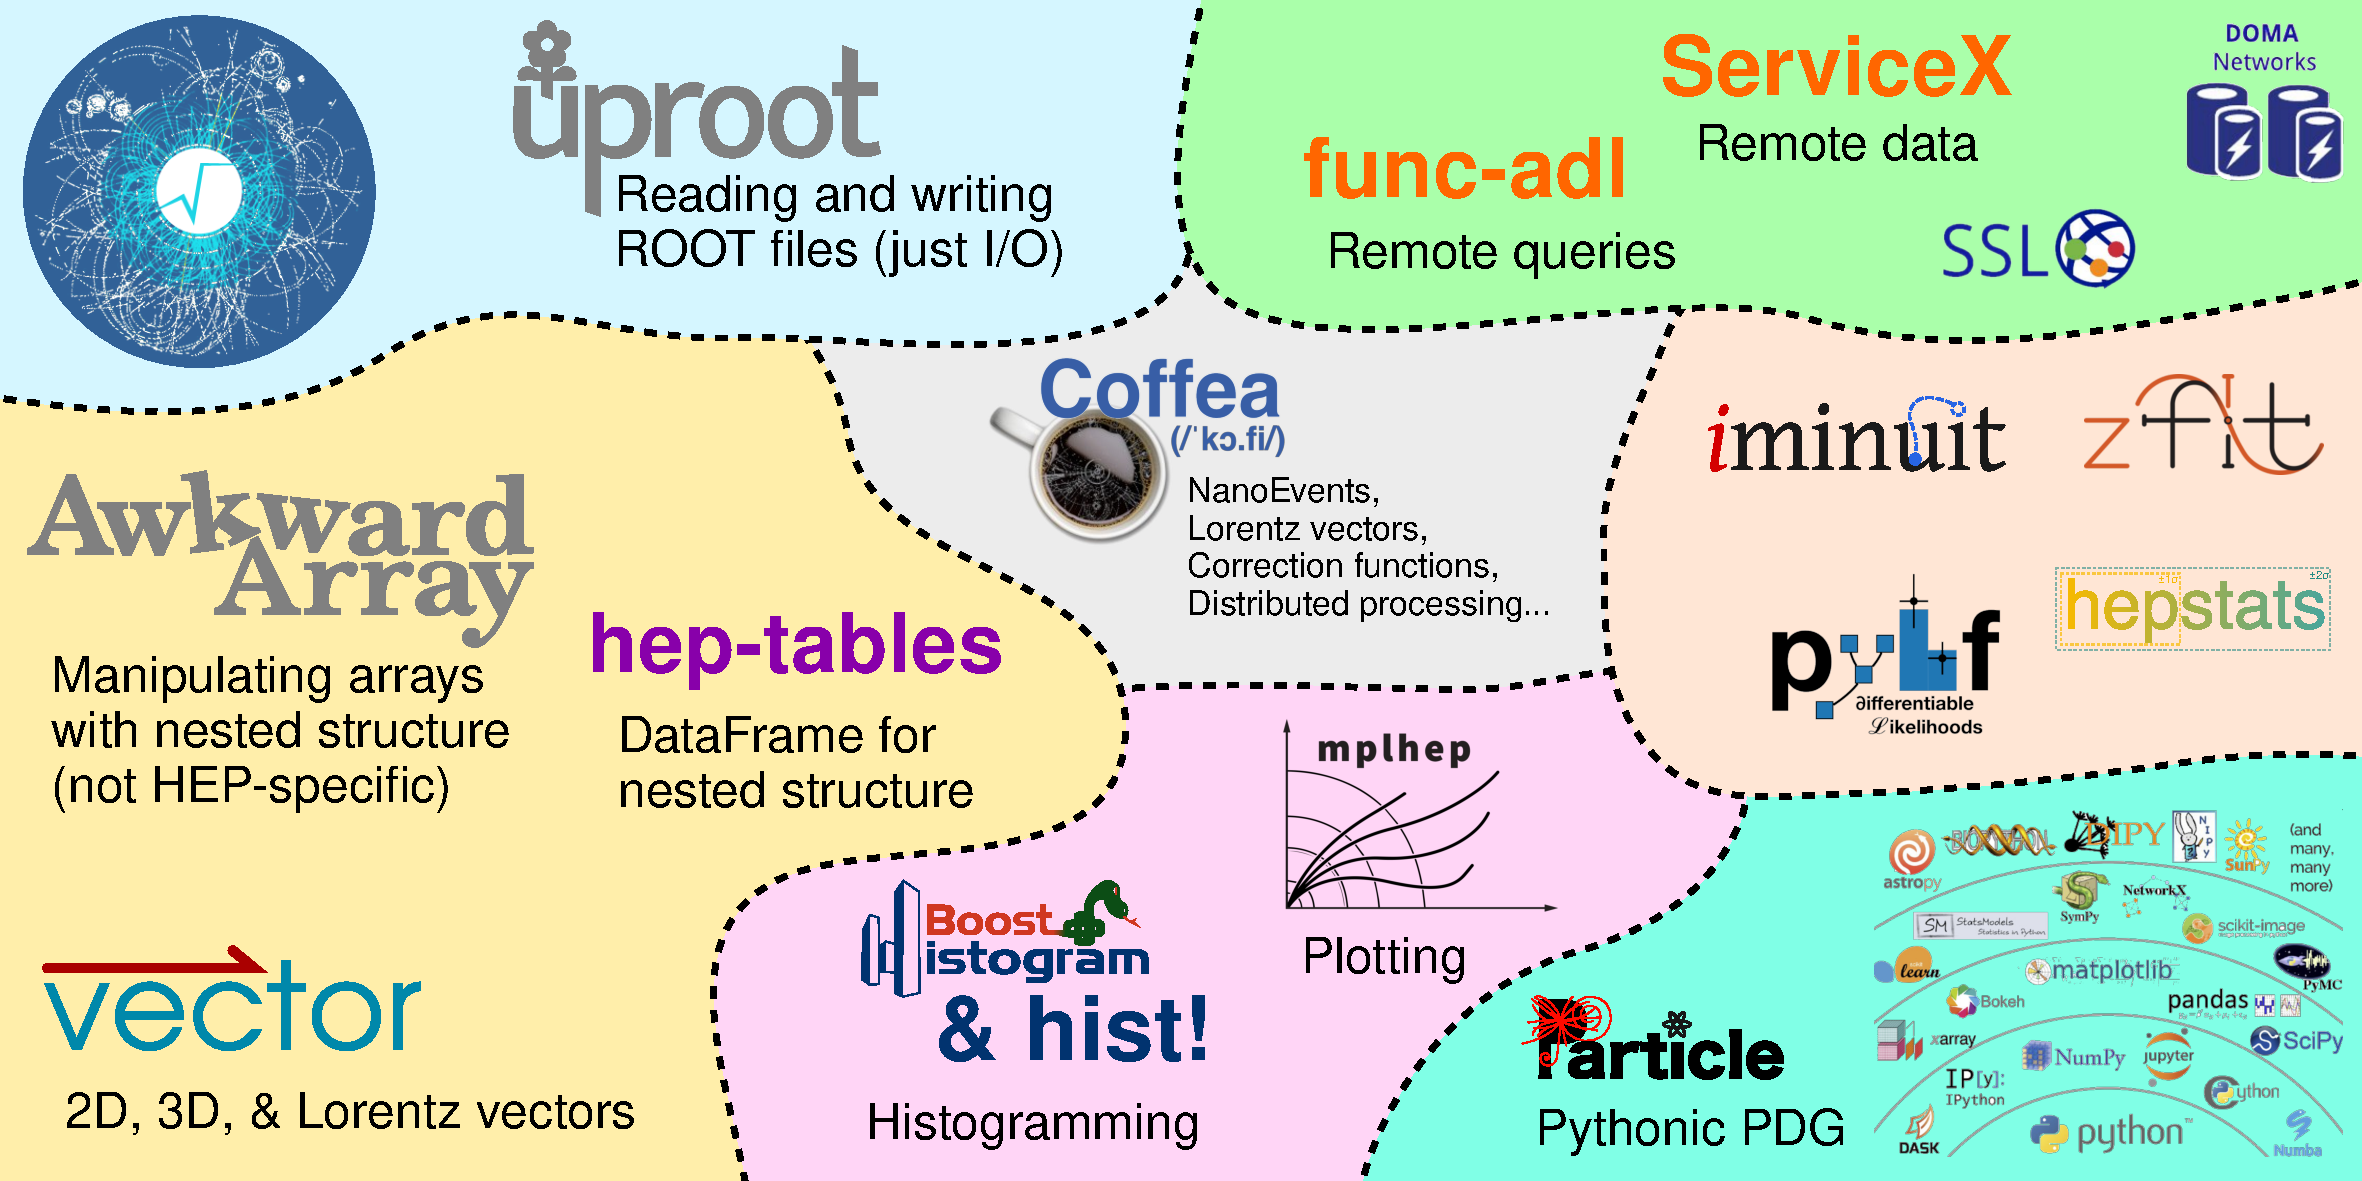
\includegraphics[width=\linewidth]{part-of-this-complete.pdf}
\end{columns}
\end{frame}

\begin{frame}[fragile]{Uproot is ROOT I/O rewritten in Python}
\vspace{0.5 cm}

\includegraphics[height=1.5 cm]{uproot-logo.pdf}

\vspace{-1.75 cm}
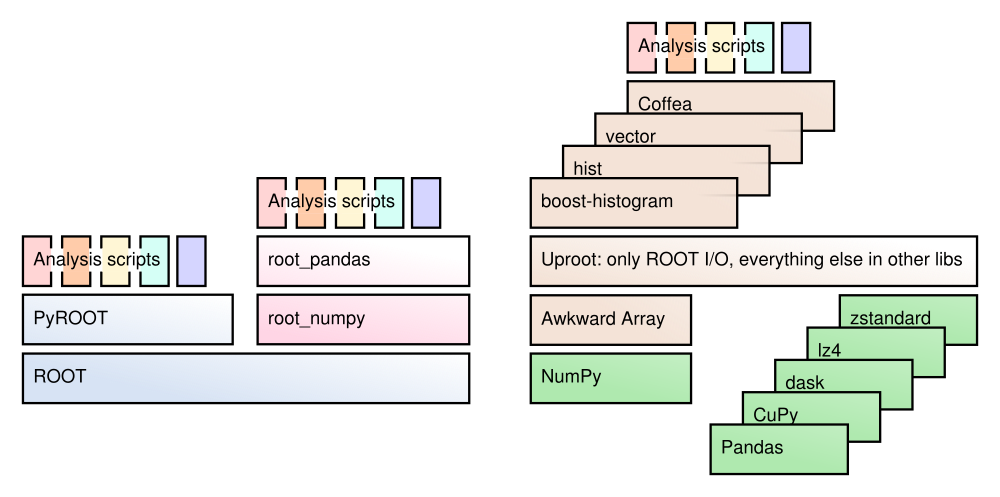
\includegraphics[width=\linewidth]{abstraction-layers.png}

\small
\vspace{-0.7 cm}
\begin{uncoverenv}<2->
\begin{minted}{python}
>>> import uproot4
>>> data = uproot4.open("file.root:Events").arrays()
\end{minted}
\end{uncoverenv}
\end{frame}

\begin{frame}[fragile]{Awkward Array is NumPy for JSON-like data}
\vspace{0.2 cm}
\hfill \mbox{
\includegraphics[height=1.5 cm]{awkward-logo.pdf}\hspace{-0.85 cm}}

\vspace{-1.5 cm}
\scriptsize
\begin{onlyenv}<1>
\begin{minted}{python}
>>> import awkward1 as ak
>>> import numpy as np
>>> 
>>> @ak.mixin_class(ak.behavior)
... class Lorentz:
...     @property
...     def pt(self):
...         return np.sqrt(self.px**2 + self.py**2)
... 
>>> array = ak.Array([{"px": 1, "py": 1, "pz": 1, "E": 1},
...                   {"px": 2, "py": 2, "pz": 2, "E": 2},
...                   {"px": 3, "py": 3, "pz": 3, "E": 3},
...                   {"px": 4, "py": 4, "pz": 4, "E": 4},
...                   {"px": 5, "py": 5, "pz": 5, "E": 5}],
...                  with_name="Lorentz")
... 
\end{minted}
\vspace{3 cm}
\end{onlyenv}
\begin{onlyenv}<2>
\begin{minted}{python}
>>> import awkward1 as ak
>>> import numpy as np
>>> 
>>> @ak.mixin_class(ak.behavior)
... class Lorentz:
...     @property
...     def pt(self):
...         return np.sqrt(self.px**2 + self.py**2)
... 
>>> array = ak.Array([{"px": 1, "py": 1, "pz": 1, "E": 1},
...                   {"px": 2, "py": 2, "pz": 2, "E": 2},
...                   {"px": 3, "py": 3, "pz": 3, "E": 3},
...                   {"px": 4, "py": 4, "pz": 4, "E": 4},
...                   {"px": 5, "py": 5, "pz": 5, "E": 5}],
...                  with_name="Lorentz")
... 
>>> array[-2]
<LorentzRecord {px: 4, py: 4, pz: 4, E: 4} type='Lorentz["px": int64, "py": int6...'>
\end{minted}
\vspace{3 cm}
\end{onlyenv}
\begin{onlyenv}<3>
\begin{minted}{python}
>>> import awkward1 as ak
>>> import numpy as np
>>> 
>>> @ak.mixin_class(ak.behavior)
... class Lorentz:
...     @property
...     def pt(self):
...         return np.sqrt(self.px**2 + self.py**2)
... 
>>> array = ak.Array([{"px": 1, "py": 1, "pz": 1, "E": 1},
...                   {"px": 2, "py": 2, "pz": 2, "E": 2},
...                   {"px": 3, "py": 3, "pz": 3, "E": 3},
...                   {"px": 4, "py": 4, "pz": 4, "E": 4},
...                   {"px": 5, "py": 5, "pz": 5, "E": 5}],
...                  with_name="Lorentz")
... 
>>> array[-2]
<LorentzRecord {px: 4, py: 4, pz: 4, E: 4} type='Lorentz["px": int64, "py": int6...'>
>>> array * 10
<Array [{px: 10, py: 10, pz: 10, ... E: 50}] type='5 * {"px": int64, "py": int64...'>
\end{minted}
\vspace{3 cm}
\end{onlyenv}
\begin{onlyenv}<4>
\begin{minted}{python}
>>> import awkward1 as ak
>>> import numpy as np
>>> 
>>> @ak.mixin_class(ak.behavior)
... class Lorentz:
...     @property
...     def pt(self):
...         return np.sqrt(self.px**2 + self.py**2)
... 
>>> array = ak.Array([{"px": 1, "py": 1, "pz": 1, "E": 1},
...                   {"px": 2, "py": 2, "pz": 2, "E": 2},
...                   {"px": 3, "py": 3, "pz": 3, "E": 3},
...                   {"px": 4, "py": 4, "pz": 4, "E": 4},
...                   {"px": 5, "py": 5, "pz": 5, "E": 5}],
...                  with_name="Lorentz")
... 
>>> array[-2]
<LorentzRecord {px: 4, py: 4, pz: 4, E: 4} type='Lorentz["px": int64, "py": int6...'>
>>> array * 10
<Array [{px: 10, py: 10, pz: 10, ... E: 50}] type='5 * {"px": int64, "py": int64...'>
>>> array.pt
<Array [1.41, 2.83, 4.24, 5.66, 7.07] type='5 * float64'>
\end{minted}
\vspace{3 cm}
\end{onlyenv}
\begin{onlyenv}<5>
\begin{minted}{python}
>>> import awkward1 as ak
>>> import numpy as np
>>> 
>>> @ak.mixin_class(ak.behavior)
... class Lorentz:
...     @property
...     def pt(self):
...         return np.sqrt(self.px**2 + self.py**2)
... 
>>> array = ak.Array([[{"px": 1, "py": 1, "pz": 1, "E": 1},
...                    {"px": 2, "py": 2, "pz": 2, "E": 2},
...                    {"px": 3, "py": 3, "pz": 3, "E": 3}],
...                   [],
...                   [{"px": 4, "py": 4, "pz": 4, "E": 4},
...                    {"px": 5, "py": 5, "pz": 5, "E": 5}]],
...                  with_name="Lorentz")
... 
>>> array[0, -1]
<LorentzRecord {px: 3, py: 3, pz: 3, E: 3} type='Lorentz["px": int64, "py": int6...'>
>>> array * 10
<Array [[{px: 10, py: 10, ... E: 50}]] type='3 * var * {"px": int64, "py": int64...'>
>>> array.pt
<Array [[1.41, 2.83, 4.24], ... [5.66, 7.07]] type='3 * var * float64'>
\end{minted}
\vspace{3 cm}
\end{onlyenv}
\begin{onlyenv}<6>
\begin{minted}{python}
>>> import awkward1 as ak
>>> import numpy as np
>>> 
>>> @ak.mixin_class(ak.behavior)
... class Lorentz:
...     @property
...     def pt(self):
...         return np.sqrt(self.px**2 + self.py**2)
... 
>>> array = ak.Array([[[{"px": 1, "py": 1, "pz": 1, "E": 1},
...                     {"px": 2, "py": 2, "pz": 2, "E": 2}],
...                    [{"px": 3, "py": 3, "pz": 3, "E": 3}]],
...                   [[]],
...                   [[{"px": 4, "py": 4, "pz": 4, "E": 4}],
...                    [],
...                    [{"px": 5, "py": 5, "pz": 5, "E": 5}]]],
...                  with_name="Lorentz")
>>> array[-1, 2, 0]
<LorentzRecord {px: 5, py: 5, pz: 5, E: 5} type='Lorentz["px": int64, "py": int6...'>
>>> array * 10
<Array [[[{px: 10, py: 10, ... E: 50}]]] type='3 * var * var * {"px": int64, "py...'>
>>> array.pt
<Array [[[1.41, 2.83], [4.24, ... [], [7.07]]] type='3 * var * var * float64'>
\end{minted}
\vspace{3 cm}
\end{onlyenv}
\end{frame}

\begin{frame}{Awkward Array has NumPy-like performance}
\vspace{0.2 cm}
\begin{columns}
\column{1.1\linewidth}
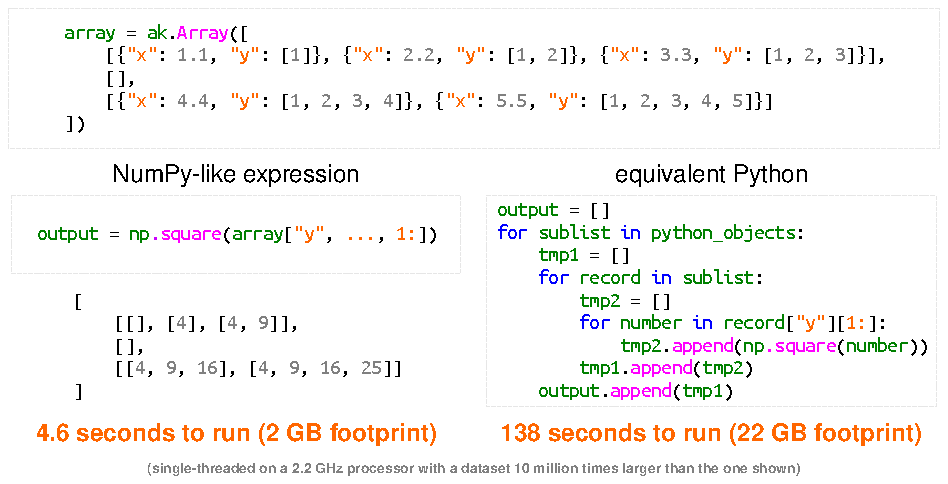
\includegraphics[width=\linewidth]{pivarski-one-slide-summary.pdf}
\end{columns}
\end{frame}

\begin{frame}{Uproot has become mainstream\ldots}
\vspace{0.75 cm}
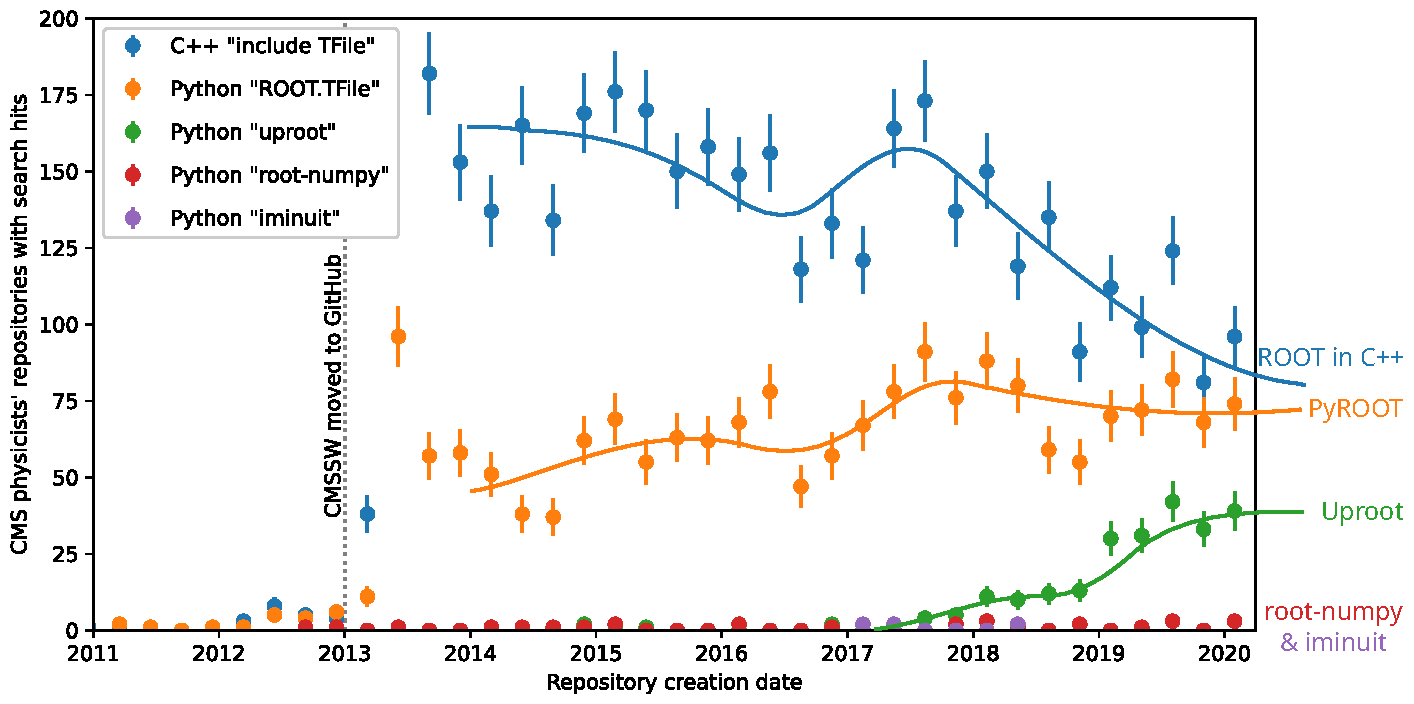
\includegraphics[width=\linewidth]{03-github-root-python.pdf}
\end{frame}

\begin{frame}{\ldots as part of a general trend toward Python that started earlier}
\vspace{0.75 cm}
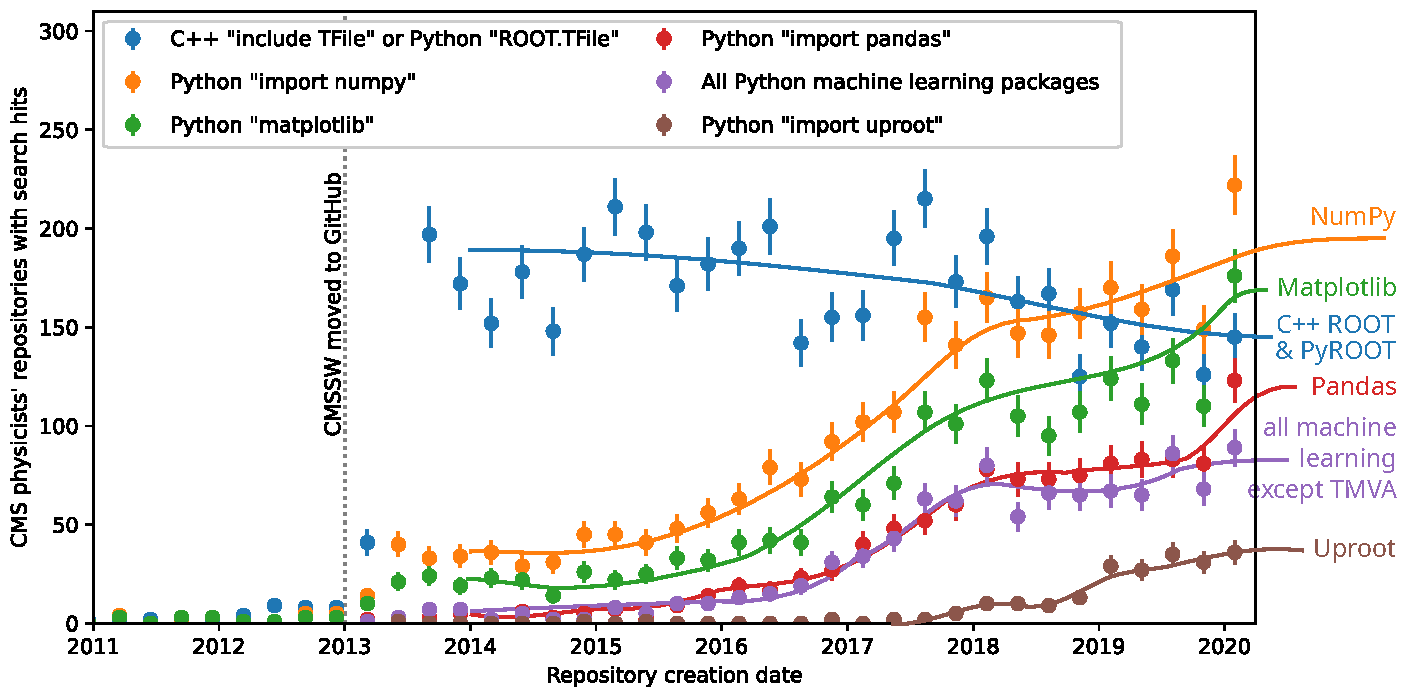
\includegraphics[width=\linewidth]{05-github-anyroot-python-machinelearning-uproot.pdf}
\end{frame}

\begin{frame}{Both libraries rewritten in 2020: new interface, better architecture}
\vspace{0.5 cm}
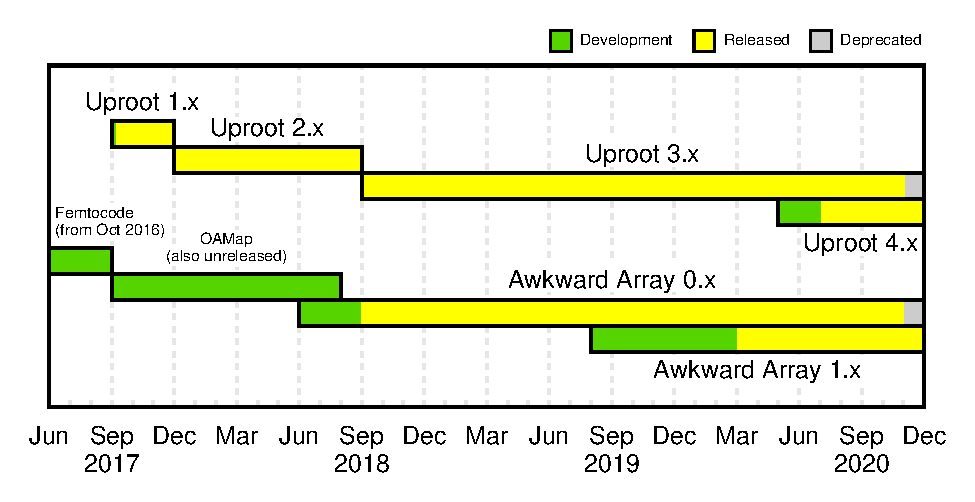
\includegraphics[width=\linewidth]{uproot-awkward-timeline.pdf}
\end{frame}

\begin{frame}{Adoption of the new libraries}
\large
\vspace{0.35 cm}

Plateaued at a small fraction of pip-installs, but significant cross-over for ``\mintinline{python}{import awkward}'' vs.\ ``\mintinline{python}{import awkward1}'' in Python files in GitHub.

\vspace{0.25 cm}
\begin{columns}
\column{1.1\linewidth}
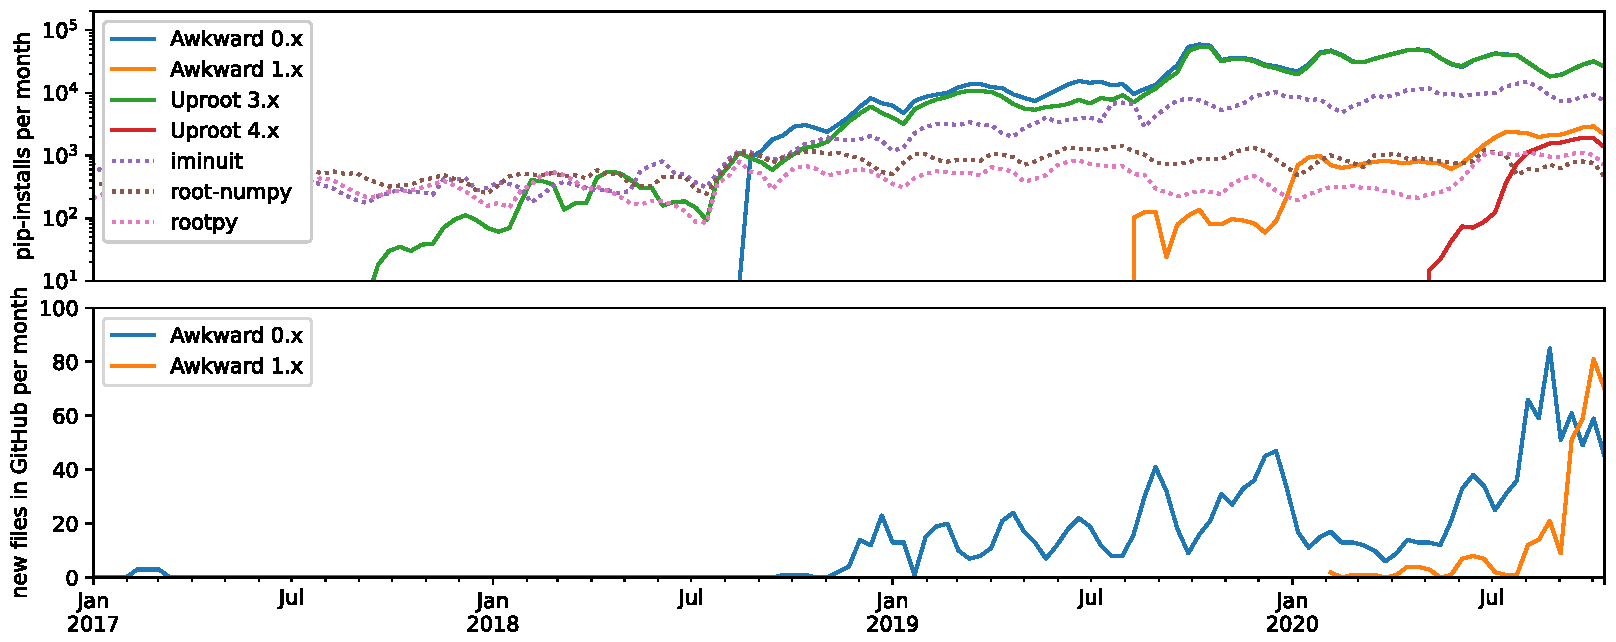
\includegraphics[width=\linewidth]{pip-github-anyone-awkward-uproot.pdf}
\end{columns}
\end{frame}

\begin{frame}{``Opt-in for new'' $\longrightarrow$ ``opt-in for old''}
\vspace{0.35 cm}
\begin{center}
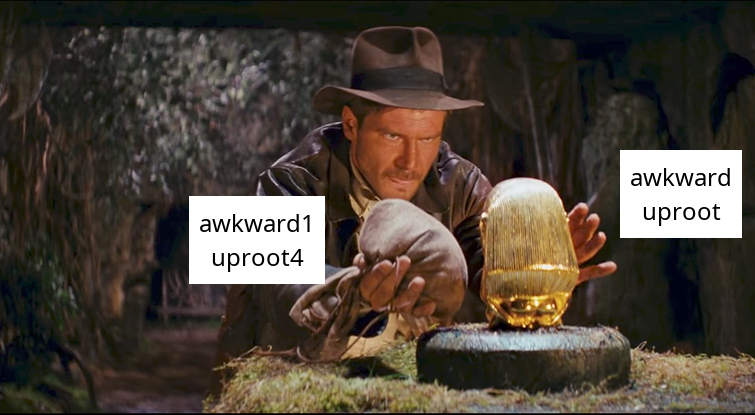
\includegraphics[width=0.8\linewidth]{Raiders-of-the-Lost-Ark-Chamber.jpg}
\end{center}
\end{frame}

\begin{frame}{``Opt-in for new'' $\longrightarrow$ ``opt-in for old''}
\large
\vspace{0.5 cm}
\begin{columns}
\column{1.07\linewidth}
\begin{tabular}{p{0.1\linewidth} | p{0.42\linewidth} | p{0.42\linewidth}}
& {\bf now} & {\bf soon} \\\hline

{\bf GitHub} & \begin{minipage}{\linewidth}
\vspace{0.15 cm}
old:

{\small\tt scikit-hep/awkward-array} {\small\tt scikit-hep/uproot}

new:

{\small\tt scikit-hep/awkward-1.0} {\small\tt scikit-hep/uproot4}
\vspace{0.15 cm}
\end{minipage} & \begin{minipage}{\linewidth}
\vspace{0.15 cm}
old:

{\small\tt scikit-hep/awkward-0.x} {\small\tt scikit-hep/uproot-3.x}

new:

{\small\tt scikit-hep/awkward-array} {\small\tt scikit-hep/uproot}
\vspace{0.15 cm}
\end{minipage} \\\hline

\begin{minipage}{\linewidth}\bf pip \&

conda\end{minipage} & \begin{minipage}{\linewidth}
\vspace{0.15 cm}
old: {\small \mintinline{bash}{install awkward uproot}}

new: {\small \mintinline{bash}{install awkward1 uproot4}}
\vspace{0.15 cm}
\end{minipage} & \begin{minipage}{\linewidth}
\vspace{0.15 cm}
old: {\small \mintinline{bash}{install awkward0 uproot3}}

new: {\small \mintinline{bash}{install awkward uproot}}
\vspace{0.15 cm}
\end{minipage} \\\hline

{\bf Python} & \begin{minipage}{\linewidth}
\vspace{0.15 cm}
old:

{\small \mintinline{python}{import awkward, uproot}}

new:

{\small \mintinline{python}{import awkward1, uproot4}}
\vspace{0.15 cm}
\end{minipage} & \begin{minipage}{\linewidth}
\vspace{0.15 cm}
old:

{\small \mintinline{python}{import awkward0, uproot3}}

new:

{\small \mintinline{python}{import awkward, uproot}}
\vspace{0.15 cm}
\end{minipage} \\\hline
\end{tabular}
\end{columns}
\end{frame}

\begin{frame}{When is ``soon''? What needs to be done first?}
\large
\vspace{0.5 cm}

\begin{description}\setlength{\itemsep}{0.5 cm}
\item[\Large Awkward Array:] \mbox{ } \\

\vspace{0.3 cm}
\begin{itemize}\setlength{\itemsep}{0.2 cm}
\item Support Python 3.9.

\item Move \mintinline{python}{libawkward.so} into its own package.

\item Awkward 0.x $\to$ Awkward 1.x cheat sheet.
\end{itemize}

\item[\Large Uproot:] \mbox{ } \\

\vspace{0.2 cm}
\begin{itemize}\setlength{\itemsep}{0.2 cm}
\item \sout{Implement file-writing in Uproot 4.}

For now, you'll have to use Uproot 3 {\it for writing only}.

\item Uproot 3.x $\to$ Uproot 4.x cheat sheet.
\end{itemize}
\end{description}

\vspace{0.65 cm}
\uncover<2->{\Large My deadline: \textcolor{darkblue}{December 1, 2020}.}
\end{frame}

\begin{frame}{Beyond that\ldots}
\large
\vspace{0.5 cm}
\begin{columns}
\column{0.85\linewidth}
{\Large Major directions:}

\vspace{0.25 cm}
\begin{itemize}\setlength{\itemsep}{0.25 cm}
\item \textcolor{darkblue}{Python ecosystem integration}: Dask, Zarr, Xarray?
\item \textcolor{darkblue}{Auto-differentiation}: JAX, elementwise, reducers
\item \textcolor{darkblue}{GPU support}: direct and through Numba (\mintinline{python}{@nb.cuda.jit})
\end{itemize}
\end{columns}
\end{frame}

\begin{frame}[fragile]{Working demo of Awkward Array on a GPU (``direct'')}
\large
\vspace{0.5 cm}
\begin{columns}
\column{1.08\linewidth}
This is \underline{\it the visible part} of Pratyush Das \& Anish Biswas's hard work this summer!

\small
\begin{minted}{python}
>>> import awkward1 as ak, numpy as np, cupy as cp
\end{minted}
\begin{minted}{python}
>>> on_cpu = ak.Array([[1.1, 2.2, 3.3], [], [4.4, 5.5]])
>>> on_cpu                           # this jagged array is on the CPU
<Array [[1.1, 2.2, 3.3], [], [4.4, 5.5]] type='3 * var * float64'>
\end{minted}
\begin{uncoverenv}<2->
\begin{minted}{python}
>>> on_gpu = ak.to_kernels(on_cpu, "cuda")
>>> on_gpu                           # this jagged array is on the GPU
<Array:cuda [[1.1, 2.2, 3.3], ... [4.4, 5.5]] type='3 * var * float64'>
\end{minted}
\end{uncoverenv}
\begin{uncoverenv}<3->
\begin{minted}{python}
>>> ak.num(on_gpu)                   # some operations work on the GPU
<Array:cuda [3, 0, 2] type='3 * int64'>
\end{minted}
\end{uncoverenv}
\begin{uncoverenv}<4->
\begin{minted}{python}
>>> np.sqrt(on_gpu)                  # performs math on GPU (using CuPy)
<Array:cuda [[1.05, 1.48, 1.82, ... 2.1, 2.35]] type='3 * var * float64'>
\end{minted}
\end{uncoverenv}
\begin{uncoverenv}<5->
\begin{minted}{python}
>>> cp.asarray(ak.flatten(on_gpu))   # stays on the GPU as a CuPy array
array([1.1, 2.2, 3.3, 4.4, 5.5])
\end{minted}
\end{uncoverenv}
\end{columns}
\end{frame}

\end{document}
